\chapter{STUDYING POLICY ATTACKS TRANSFERABILITY AGAINST DEFENDED POLICIES}
\label{sec:exp2}

This section reports the results of the second of the three experiments included in this thesis. It evaluates the same policy attacks but this time attacking defended policies. It still focuses on attacks' transferability and shows some interesting findings

\section{Studying policy attacks transferability against defended policies}
This experiment can be viewed as the direct extension of the previous one showed in section \ref{sec:exp1}. This time, all the policies under attack have been defended with FGSM adversarial training and the goal of this work is to study the transferability of some policy attack methods against defended policies. To draw the {\it reward vs accuracy} curve of the evaluated methods, adversarial training has been conducted with a value of \(epsilon\) slightly inferior to the \(epsilon\) that defines the distance of the adversarial perturbations. In this way, it's more clear the effect of the attacks against the defended policies. The experiments have been conducted on the same three reinforcement learning algorithms adopted in section \ref{sec:exp1}: DQN, A2C, and PPO with policies trained only on the environment of Pong. In addition, the policy attack methods that have been compared include:
\begin{itemize}
    \item Uniform attack;
    \item Strategically-timed attack.
\end{itemize}
The reason why we have chosen only uniform attack and strategically-timed attack is to test one method based on untargeted image attacks and the second one based on targeted image attacks. Given the previous results, these two methods are enough to have a general idea of the robustness of an algorithm. Thus, the scope of the experiment has then been reduced to 2 policy attacks.

\subsection{Experiments settings}
\subsubsection{Defenses hyper-parameters}
\label{sec:exp2-params}
All policies have been protected with FGSM adversarial training applied over the same policies trained normally. This means that adversarial training has not been applied on models training from scratch but it has been applied on models that had already learned a working policy. Once again, FGSM has been chosen because of its speed over iterative methods. Many works such as \cite{li2020understanding} cite that during FGSM adversarial training, the robust accuracy of the model would suddenly drop to almost 0\% after a certain point. This phenomenon was commonly referred to as {\it catastrophic overfitting}. The reason for this phenomenon is that, since FGSM is a simple attack, the model learns to fool the FGSM attacks by inducing obfuscated gradient, thus making the gradient no longer a useful direction for constructing adversarial examples. However, the way adversarial training is applied to reinforcement learning algorithms is a little different from the standard adversarial training applied to image classification models and not much is known about catastrophic overfitting under reinforcement learning adversarial training. The second important point to remark is that during adversarial training perturbations have been crafted with \(epsilon=0.01\) and, when attacking, policies' noise \(epsilon\) has been raised to 0.05. All distances are computed under \(l_\infty\) norm. This discrepancy is to make sure that the adversarial perturbations can break the defended policies so as to draw more understandable {\it reward vs attack frequency} curves. As we can see from table \ref{table:adv_def}, adversarial training works well enough that adversarial observations crafted with the same perturbation distance used during training are not capable to fool the defended model. Moreover, the configuration of the algorithms during adversarial training is the same used in the previous experiments. The only small difference regards DQN, since the base policy has already been trained, the algorithm doesn't need much exploration during adversarial training. Consequently, the exploration noise has been held fixed to 0.05 for the whole process of training. The training process has been conducted over 2.5M frames for DQN and 5M frames for A2C and PPO. During adversarial training, the network is given in input adversarial observations with probability 0.5 and clean observations with the same probability so as to not forget how to deal with clear observations. In another experiment where adversarial training was conducted only using adversarial observation, the trained policy worked very well in presence of perturbations but seemed to predict random actions in correspondence to clear observations.

\begin{table}
  \centering
  \caption{Average reward scored by three policies trained with DQN, A2C and PPO respectively and defended with FGSM Adversarial training with \(epsilon=0.01\) under \(l_\sameinfty\) norm.}
  \begin{tabular}{cccc}
    \toprule
    Observations & DQN (FGSM-AT) & A2C (FGSM-AT) & PPO (FGSM-AT) \\
    \midrule
     Clear & 19.6 & 18.8 & 19.7 \\ 
     Adversarial & 19.4 & 17.9 & 18.7 \\
    \bottomrule
  \end{tabular}
  \label{table:adv_def}
\end{table}

\subsubsection{Image adversarial attacks settings}
The configuration of the white-box attacks is identical to the one used in the previous experiment in section \ref{sec:exp1}. In this way, we provide a fair comparison with the curves obtained when attacking undefended policies.

\section{Results}
The next two sections show the {\it reward vs. attack frequency} curves of uniform attack and strategically-timed attack under a fixed threat model so to measure their effectiveness and their transferability against policies and algorithms protected with adversarial training. When analyzing the obtained results, sometimes we may refer to the curve of the policy attacked without transferability as baseline policy. In addition, we may sometimes intend as attacking with a surrogate policy or attacking with a surrogate algorithm as crafting adversarial perturbations exploiting a surrogate policy/algorithm to attack the target policy. Since we want to focus on studying attack transferability and that the adversary is cheating by crafting perturbations that are stronger than the ones crafted by adversarial training, we will ignore the absolute performance of the curves but we will focus on their relative distance between each other and the baseline. In fact, table \ref{table:adv_def} shows that, even if all observations were adversarial, that is when the attack frequency is equal to 1, crafting adversarial observations with the same perturbation strength used during training the average reward wouldn't be lowered too much respect to not performing any attack at all.

\subsection{Attacking adversarially trained Pong-DQN}
The curves obtained attacking Pong-DQN with uniform and strategically-timed attack are shown in figure \ref{figure:pong-dqn-def}. The first thing we can observe is that the curves of the baseline and of the surrogate policy are practically identical, this indicates that uniform attack benefits an excellent policy transferability. Similarly, also the curve for the algorithm transferability of A2C stays close to the baseline, thus showing a good transferability. This phenomenon is more clear in correspondence to higher attack frequencies. Only attacks crafted with PPO seem to be less capable to fool the target policy. In fact, its corresponding curve keeps a distance of about 10 points with respect to the baseline in the evaluated frequency interval. Analyzing strategically-timed attack, we can surprisingly note that attacking with the surrogate policy yields even better results than directly attack the target policy. Overall, PPO is the worst algorithm when crafting adversarial perturbations and it is always a safer choice to craft them on a policy trained with the same algorithm. 

\begin{figure}
  \centering
  \subcaptionbox{Uniform attack\label{fig:subfig-a}}
    {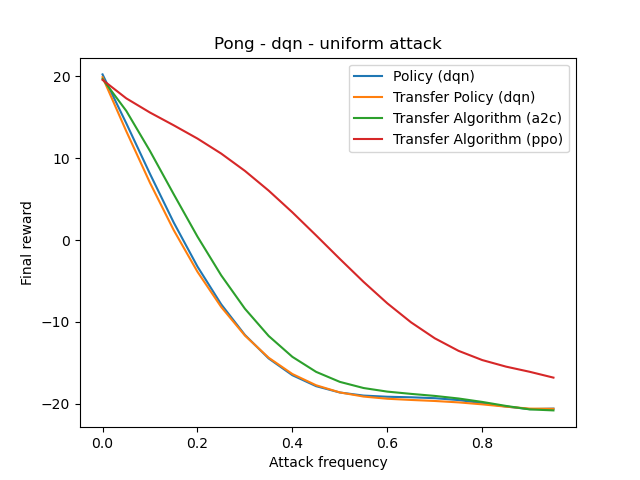
\includegraphics[width=0.49\linewidth]{images/exp2/dqn-pong-uniform.png}}
  \subcaptionbox{Strategically-timed attack\label{fig:subfig-b}}
    {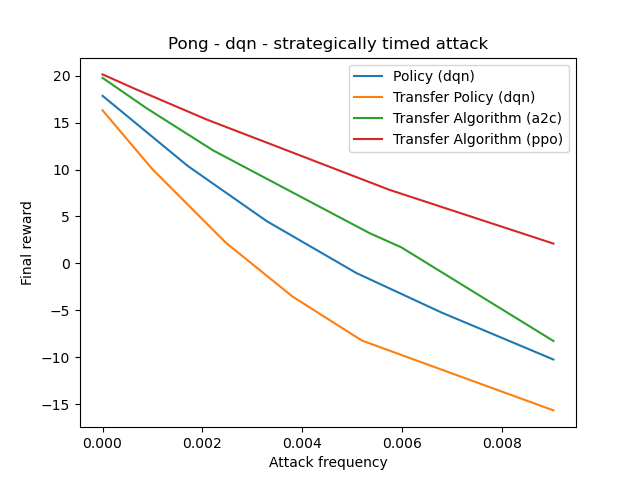
\includegraphics[width=0.49\linewidth]{images/exp2/dqn-pong-strategically_timed.png}}
  \caption{The {\it reward vs. attack frequency} curves of 2 policy attacks with FGSM under the \(l_\infty\) norm attacking a Pong-DQN policy defended with FGSM adversarial training with \(epsilon=0.01\). Attacks have been performed with \(epsilon=0.05\) to show the drop in reward as the attack frequency increases.}
  \label{figure:pong-dqn-def}
\end{figure}

\subsection{Attacking adversarially trained Pong-A2C}
The curves resulting from attacking Pong-A2C are depicted in figure \ref{figure:pong-a2c-def}. The chart presents a similar pattern to the chart of the corresponding DQN version. In fact, the curves relative to policy transferability and DQN algorithm transferability remain close to the baseline. Attacks crafted on PPO result to be less effective with its curve remaining about 5 points over the other curves. Regarding strategically-timed attack, the curve of the surrogate A2C policy is still very close to the baseline of A2C. In this case, the perturbations crafted on DQN are the ones that perform the worst followed by A2C but still maintaining only a few points of difference with respect to the baseline. 

\begin{figure}
  \centering
  \subcaptionbox{Uniform attack\label{fig:subfig-a}}
    {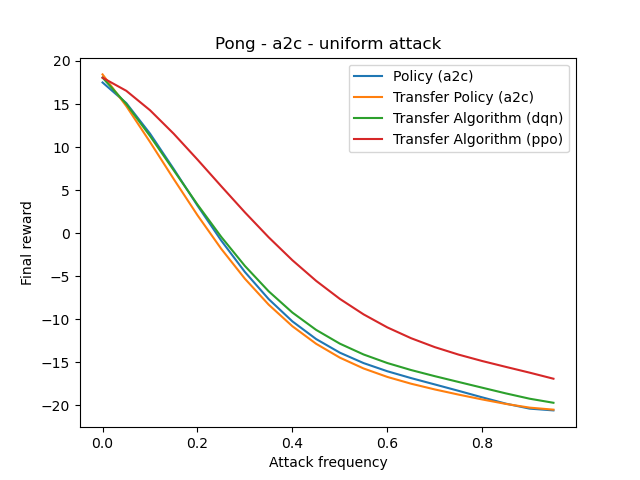
\includegraphics[width=0.49\linewidth]{images/exp2/a2c-pong-uniform.png}}
  \subcaptionbox{Strategically-timed attack\label{fig:subfig-b}}
    {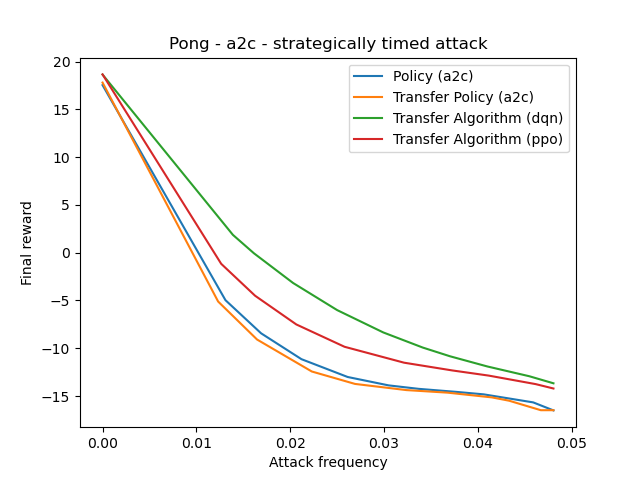
\includegraphics[width=0.49\linewidth]{images/exp2/a2c-pong-strategically_timed.png}}
  \caption{The {\it reward vs. attack frequency} curves of 2 policy attacks with FGSM under the \(l_\infty\) norm attacking a Pong-A2C policy defended with FGSM adversarial training with \(epsilon=0.01\). Attacks have been performed with \(epsilon=0.05\) to show the drop in reward as the attack frequency increases.}
  \label{figure:pong-a2c-def}
\end{figure}

\subsection{Attacking adversarially trained Pong-PPO}
The curves obtained from attacking Pong-PPO are represented in figure \ref{figure:pong-ppo-def}. Attacks crafted with any policy show a good transferability for the uniform attack such that choosing any surrogate model to generate adversarial observations would yield performance similar to attacking the victim model. PPO policy is a little more robust against strategically-timed attack which presents more spaced curves. More specifically, transferability over A2C works better than transferability over DQN, and transferability over PPO is the one that yields performance most similar to the baseline.

\begin{figure}
  \centering
  \subcaptionbox{Uniform attack\label{fig:subfig-a}}
    {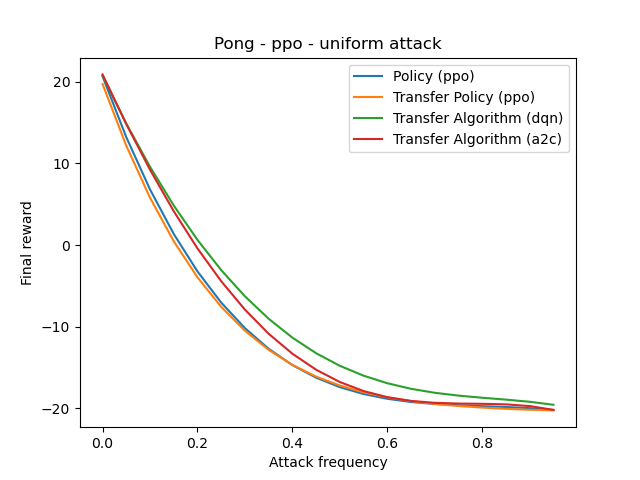
\includegraphics[width=0.49\linewidth]{images/exp2/ppo-pong-uniform.png}}
  \subcaptionbox{Strategically-timed attack\label{fig:subfig-b}}
    {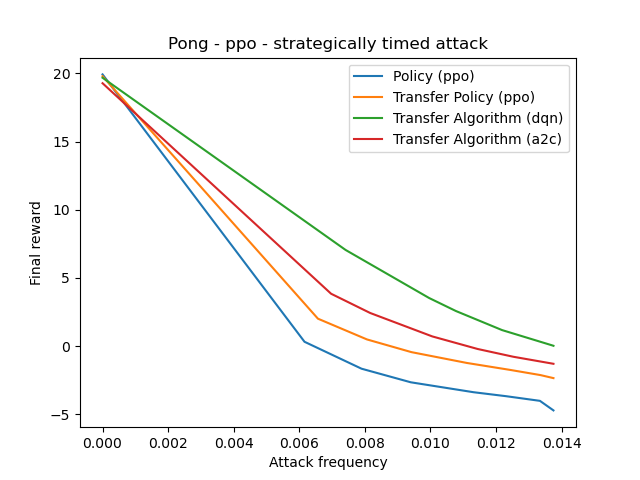
\includegraphics[width=0.49\linewidth]{images/exp2/ppo-pong-strategically_timed.png}}
  \caption{The {\it reward vs. attack frequency} curves of 2 policy attacks with FGSM under the \(l_\infty\) norm attacking a Pong-PPO policy defended with FGSM adversarial training with \(epsilon=0.01\). Attacks have been performed with \(epsilon=0.05\) to show the drop in reward as the attack frequency increases.}
  \label{figure:pong-ppo-def}
\end{figure}

\section{Findings}
This section provides further analyses about the policies that have been evaluated. In particular, it makes some conclusions about the performance obtained when attacking with similar policies and with similar algorithms.

\subsection{Performance of similar policies}
In most of the charts showed in this section as well as in section \ref{sec:exp1}, the attacks crafted on the surrogate policies trained with the same algorithm of the victim policy own a better transferability than the attacks crafted on the policies trained with different algorithms. We can then conclude that attacking similar policies is more effective than attacking different algorithms. This is the same property observed when attacking common image classificators: attacking a surrogate model with the same architecture provides better results than attacking models with different architectures.

\subsection{Performance of similar algorithms}
Among the three evaluated algorithms, DQN is off-policy, which means that it learns in a different way than A2C and PPO which are on-policy. Moreover, A2C and PPO are substantially similar with the introduction of the clipping hyper-parameter being a major difference. Hence, as we can see from the charts of the experiments in both this chapter and in the previous one, a policy trained with A2C can be more easily attacked with PPO rather than with a policy trained with DQN. On the other way around, a policy trained with PPO can be more easily attacked with A2C. Thus algorithm transferability is more effective when the surrogate policy is trained with an algorithm similar to the algorithm used to train the victim policy.